\section{Theorie}
\label{sec:Theorie}

Die Zielsetzung dieses Versuchs ist es die Aufspaltung von Spektrallinien von Atomen unter dem Einfluss eines Magnetfeldes zu untersuchen. Dabei wird die Aufspaltung der roten und blauen Linie von Cd-Atomen untersucht.

\subsection{Drehimpuls und magnetisches Moment für Elektronen}

Allgemein besitzen die Hüllenelektronen von Atomen einen Bahndrehimpuls $\vec{l}$ und einen Spin $\vec{s}$ sowie die Quantenzahl $l$ und den Spin $s$. Für Elektronen gilt $s = \sfrac{1}{2}$. Für die Bahndrehimpulsquantenzahl gilt $l \in \{0, 1, 2, \ldots , n-1\}$. Dabei ist $n \in \symbb{N}$ die Hauptquantenzahl. Dazu kommt die magnetische Quantenzahl $m \in \{-l, -l+1, \ldots, l-1, l\}$. Damit können die magnetischen Momente der Elektronen als

\begin{align}
    \lvert \vec{\mu_l} \rvert &= \mu_\text{B} \sqrt{l(l+1)} = g_l \mu_\text{B} \frac{l}{\hbar}
    \label{eqn:magn_mom_l} \\
    \lvert \vec{\mu_s} \rvert &= \mu_\text{B} \sqrt{s(s+1)} = g_s \mu_\text{B} \frac{s}{\hbar} 
    \label{eqn:magn_mom_s}
\end{align}

geschrieben werden. Dabei ist $\mu_B = -\frac{e_0 \hbar}{2 m_0}$ das Bohrsche Magneton und die Faktoren $g_{i}$ mit $i \in \{j,l,s\}$ heißen Landé-Faktoren. Die Landé-Faktoren lassen sich mit der Gleichung
\begin{equation}
    g_{j} = 1 + \frac{j(j+1) + s(s+1) - l(l+1)}{2j(j+1)}
    \label{eqn:lande}
\end{equation}
berechnen. Das heißt es gilt $g_l = 1$ für $s = 0$ (also für einen Gesamtspin von 0) und $g_s = 2$ für $l = 0$.

\subsection{Auswahlregeln}

Die Auswahlregeln bestimmen welche optischen Übergänge zwischen den Energieniveaus erlaubt sind. Hier ist die Regel, dass die Änderung der Drehimpulsquantenzahl $\Delta l = \pm 1$ und, dass die Änderung der magnetischen Quantenzahl beim Übergang $\Delta m = 0$ oder $\Delta m = \pm 1$ betragen muss.
Für eine Änderung der Magnetquantenzahl von $\Delta m = \pm 1$ werden zirkular $\sigma^{+}$- oder $\sigma^{-}$-polarisierte Photonen emittiert, während für $\Delta m = 0$ linear $\pi$-polarisiertes Licht emittiert wird.

\subsection{Der Zeeman-Effekt}

Der Zeeman-Effekt beschreibt die Aufspaltung von Spektrallininen unter dem Einfluss eines externen Magnetfeldes. Diese Aufspaltung ensteht wegen der Aufspaltung der Energieniveaus durch das Magnetfeld. \\
Für den Gesamtdrehimpuls kann das magnetische Moment mit der Formel
\begin{equation}
    \vec{\mu_J} = - m g_j \mu_\text{B} \vec{e_z} \ .
\end{equation}
beschrieben werden. Dazu gilt allgemein im magnetischen Feld 
\begin{equation}
    E_\text{mag} = - \vec{\mu_J} \cdot \vec{B} = m g_J \mu_\text{B} |\vec{B}| \: .
    \label{eqn:energie}
\end{equation} 

Mit diesem magnetischen Moment kann man also für die Energiedifferenzen zwischen den aufgespaltenen Energieniveaus, welche für den Zeeman-Effekt sorgen, schreiben: 
\begin{equation}
    \symup{\Delta} E = g_j \symup{\Delta} m \mu_\text{B} \lvert \vec{B} \rvert 
    \label{eqn:energiediff}
\end{equation}


\subsubsection{Der normale Zeeman-Effekt}

Der normale Zeeman-Effekt tritt auf, wenn der Gesamtspin des Systems $S = 0$ beträgt. Das heißt, dass für den Landé-Faktor nach \autoref{eqn:lande} immer $g_j = 1$ gilt.
Es ergibt sich nach Gleichung \eqref{eqn:energiediff} die Verschiebung der Energieniveaus um

\begin{equation}
    \Delta E = \symup{\Delta} m \mu_\text{B} |\vec{B}|\: .
\end{equation}
\newline
\noindent
Beim Cadmium ist der normale Zeeman-Effekt bei der roten Linie bei $\lambda = \SI{643.8}{\nano\meter}$ zu beobachten. Das Termschema für den dazu passenden Übergang von $^1D_2 \leftrightarrow ^1P_1$ ist in \autoref{fig:rot1} dargestellt.

\begin{figure}[H]
    \centering
    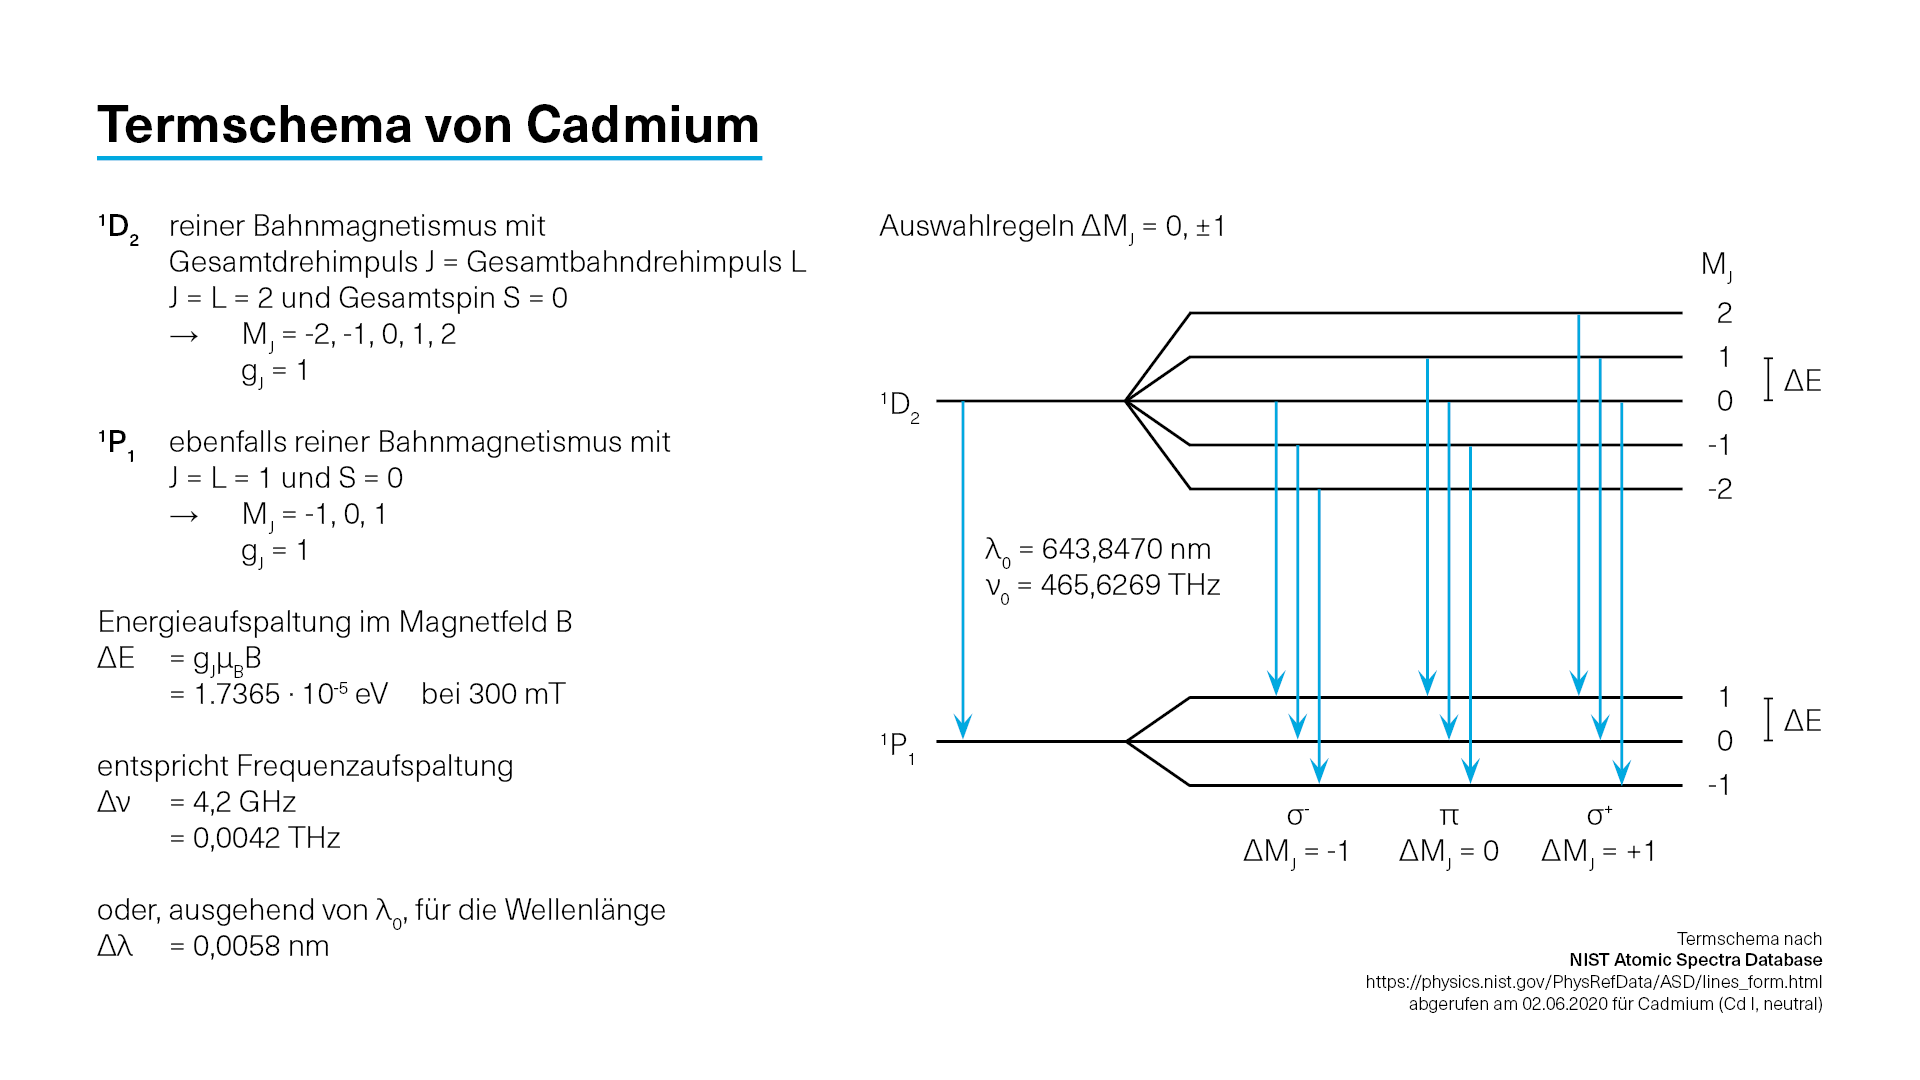
\includegraphics[width=\textwidth]{graphics/termschema_Cd_rot.png}
    \caption{Termschema für die rote Cd-Linie bei $\lambda = \SI{643.8}{\nano\meter}$. \cite{rot}}
    \label{fig:rot1}
\end{figure}

Es ist zu sehen, dass drei $\sigma^{+}$-, drei $\sigma^{-}$ sowie drei $\pi$- Übergänge möglich sind. Je nach $\symup{\Delta} m$ ergibt sich für die Energieverschiebung dann:
\begin{equation*}
    \symup{\Delta} E =
    \begin{cases}
        - \mu_\text{B} \lvert \vec{B} \rvert & \text{für } \symup{\Delta} m = -1 \\
        0 & \text{für } \symup{\Delta} m = 0 \\
        \mu_\text{B} \lvert \vec{B} \rvert & \text{für } \symup{\Delta} m = +1
    \end{cases}
\end{equation*}

\subsubsection{Der anormale Zeeman-Effekt}

Beim anormalen Zeeman-Effekt werden Übergänge mit einem Gesamtspin von $S \neq 0$ betrachtet. Das heißt, dass die Übergänge und insbesondere die Landé-Faktoren vom Spin abhängig sind. Die Formeln für die Energiedifferenz und die Landé-Faktoren werden daher zu 
\begin{align}
    \symup{\Delta} E &= g_{ab} \mu_\text{B} \lvert \vec{B} \rvert \ 
    \label{eqn:energiedifferenz}\\
    g_{ab} &= m_a g_a - m_b g_b
    \label{eqn:lande_anormal}
\end{align}
angepasst.
\newline
\noindent
Für Cadmium ist der anormale Zeeman-Effekt bei der blauen Linie bei $\lambda = \SI{480}{\nano\meter}$ zu beobachten. Das entsprechende Termschema für den Übergang $^3S_1 \leftrightarrow ^3P_1$ ist in \autoref{fig:blau} dargestellt.

\begin{figure}[H]
    \centering
    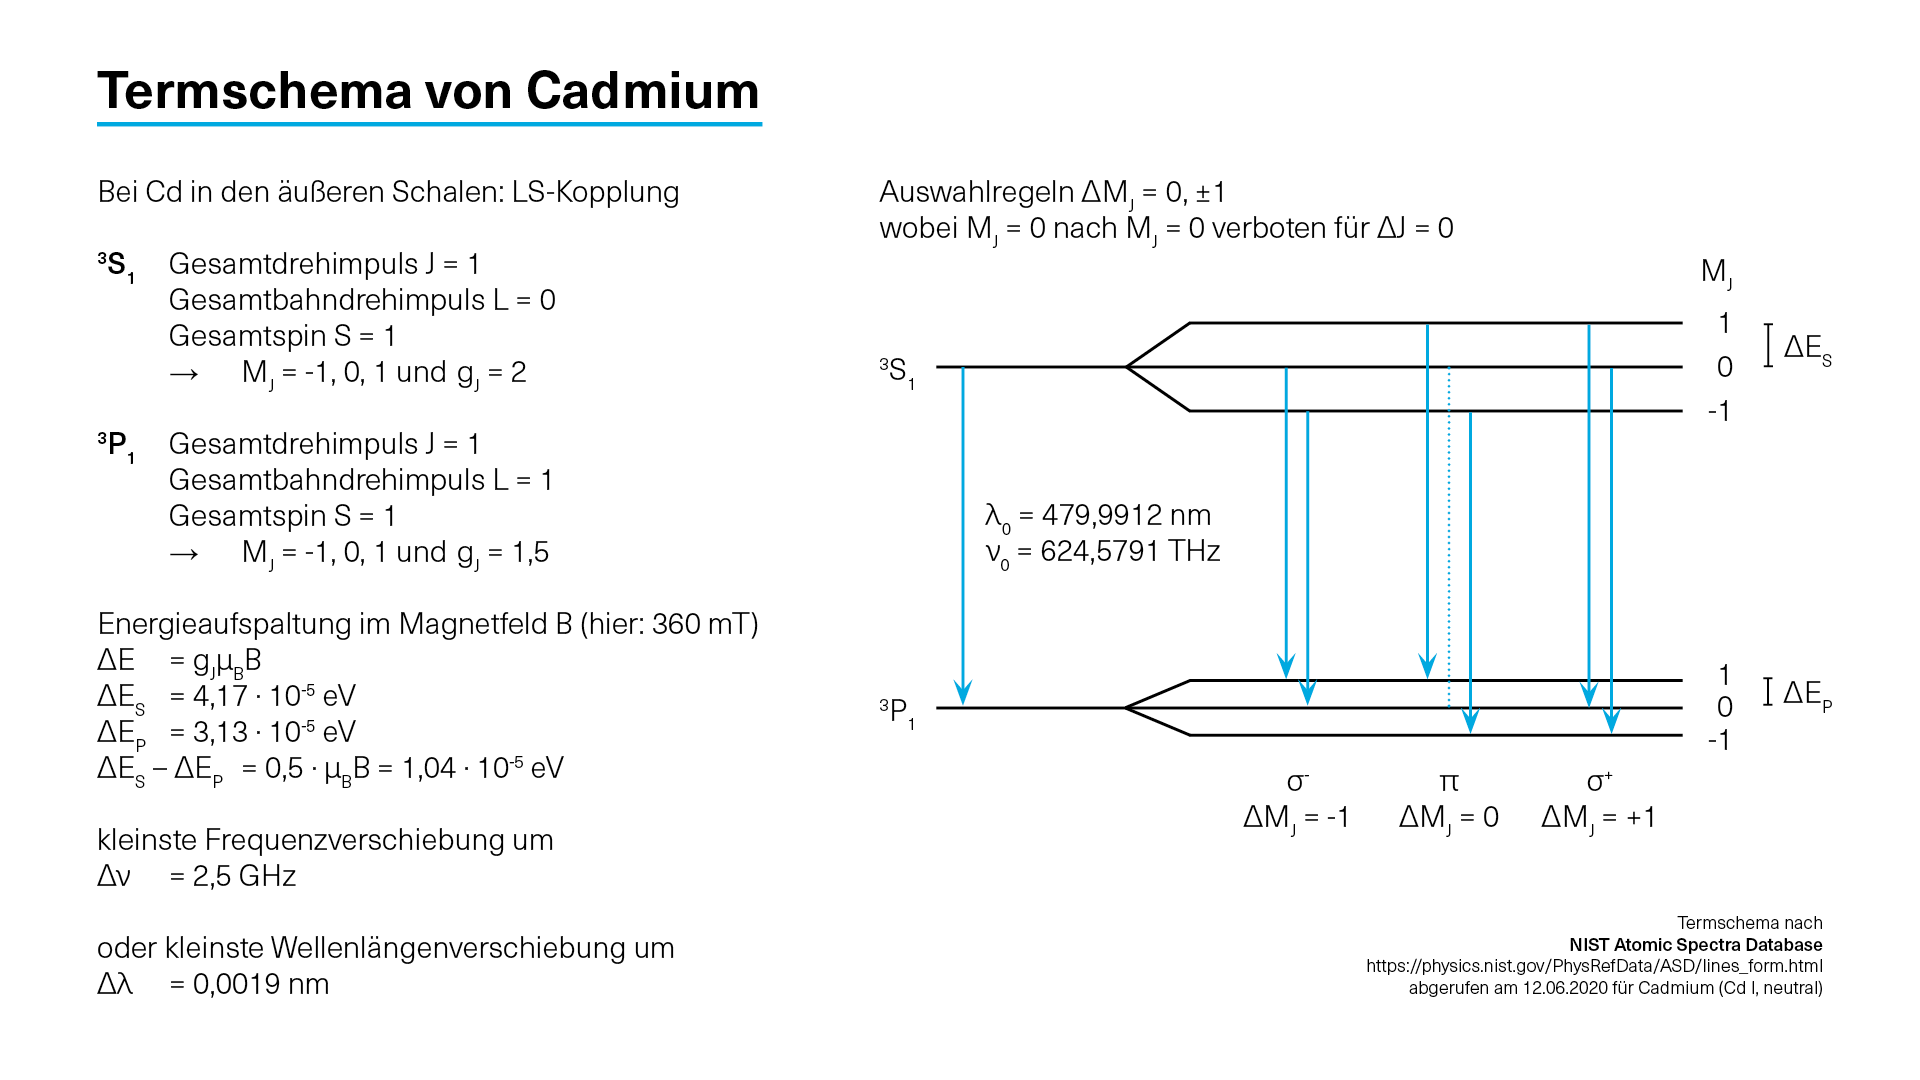
\includegraphics[width=\textwidth]{graphics/Termschema_Cd_tuerkis.png}
    \caption{Termschema für die blaue Cd-Linie bei $\lambda = \SI{480}{\nano\meter}$. \cite{blau}}
    \label{fig:blau}
\end{figure}

Es werden die bereits beschriebenen optischen Auswahlregeln ($\Delta l = \pm 1$  und $\Delta m = 0$ oder $\Delta m = \pm 1$) genutzt, sodass, wie in \autoref{fig:blau} zu sehen ist, zwei $\sigma^{+}$-, zwei $\sigma^{-}$ und zwei $\pi$- Übergänge möglich sind.